\graphicspath{{./img/}}

Nuestra Hipotesis a la hora de experimentar, es que, utilizar el modelo SIMD con operaciones SSE, nos da una mayor performance a la hora de desarrollar nuestros algoritmos. El hecho de poder procesar varios datos a la misma vez, nos permite ahorrarnos tiempo de ejecucion y cantidad de iteraciones en nuestros algoritmos.
Realizamos distintas corridas de nuestro codigo, tanto en ASM, como en C con las correspondientes optimizaciones que nos permite el compilador. De esta manera pudimos respaldar nuestra hipotesis con resultados concretos.

\subsection{solver\_lin\_solve}

El objetivo a alcanzar fue que la implementacion de solver$\_$lin$\_$solve en asm tarda menos que alguna de las implementaciones de c en O, O2 u O3. Para ello se hizo un experimento en el cual para un nivel de optimizacion ejecuto 1000 veces la funcion en asm y en c para tres tamaños diferentes de matrices. Por cada llamado se le va a tomar el tiempo, es decir la cantidad de clocks que le toma en ejecutarse. Ademas para evitar por ejemplo que los clocks que le toma a la funcion en asm para la matriz de tamaño 256 sean altos en principio y luego bajen mucho, lo que se hace es llamar a la funcion de asm con un tamaño de matriz despues a la de c con un tamaño de matriz diferente e ir intercalando los llamados sucesivamente. 
El valor del parametro 'b' se lo dejo fijo porque no lo usa solver$\_$lin$\_$solve ya que se lo pasa a solver$\_$set$\_$bnd. El valor de 'a' y 'c' se los dejo fijos, ya que solo multiplican y dividen valores para modificar una de las matrices que se le pasan por parametreo a solver$\_$lin$\_$solve.
Para un tamaño de matriz en un fichero estaran los clocks que le toma ejecutar a la funcion de c en O0, abajo siguen los clocks de O2 y por ultimo estan los de O3. Los clocks que le toman a la funcion de asm se guarda de la misma forma que c.
  

\begin{figure}[h]
  \centering
    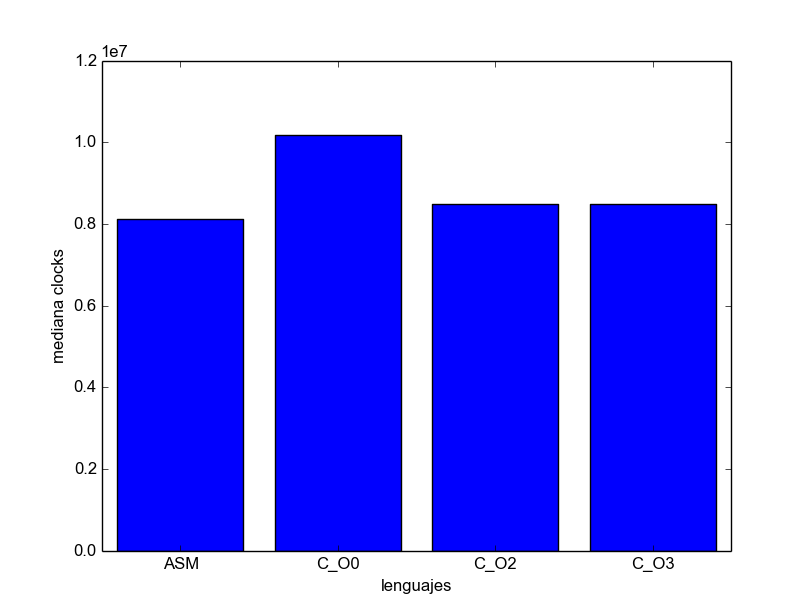
\includegraphics[width=.6\linewidth]{Matriz_128.png}
    \caption{Performance para Matriz 128x128}
    \label{fig:M128}
\end{figure}

\pagebreak

\begin{figure}[h]
  \centering
    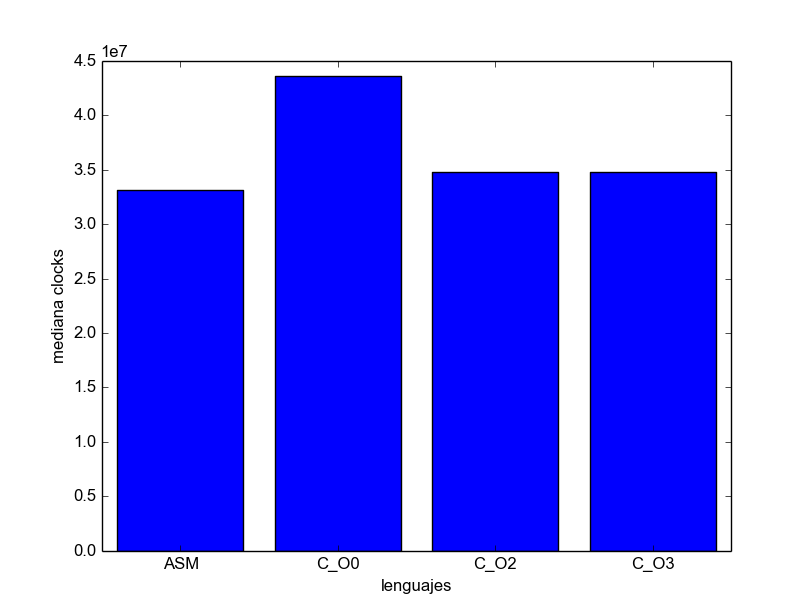
\includegraphics[width=.6\linewidth]{Matriz_256.png}
    \caption{Performance para Matriz 256x256}
    \label{fig:M256}
\end{figure}

\begin{figure}[h]
  \centering
    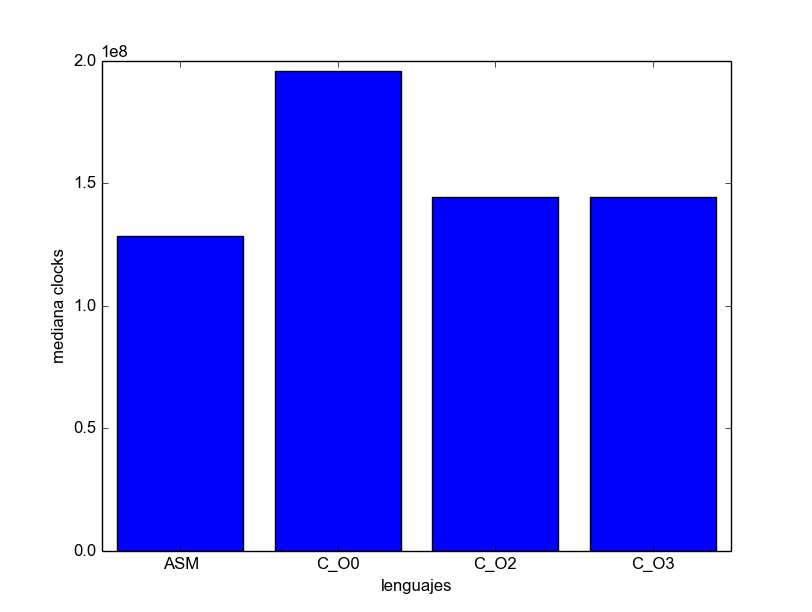
\includegraphics[width=.6\linewidth]{Matriz_512.png}
    \caption{Performance para Matriz 512x512}
    \label{fig:M512}
\end{figure}

\newpage

\subsection{solver\_set\_bnd}

En solver$\_$set$\_$bnd se hicieron 4 gráficos para comparar ASM y C con los distintos tamaños, que son iguales a los tamaños de las imágenes de la cátedra. El solver tiene 2 matrices de floats, que son las que utilizamos para hacer los experimentos en este caso. Si bien el $b$ se cambió en cada iteración para que el procesador no cachee los experimentos y tengamos tiempos medianamente razonables, no se graficó ya que no influye en el algoritmo.
Los pasos para los experimentos fueron los siguientes:
Por cada tamaño, en total 6, se hicieron 750 iteraciones. En cada iteración se corre un código diferente(ASM, C), con una matriz diferente (v o u) y con b diferente (0, 1, 2) a la iteración inmediata anterior. En todos los siguientes casos se utiliza la mediana como mediana.
Todo esto se vuelca en un csv, donde por python, con las bibliotecas NumPy y Matplotlib terminamos haciendo los gráficos. 

\begin{figure}[h]
  \centering
    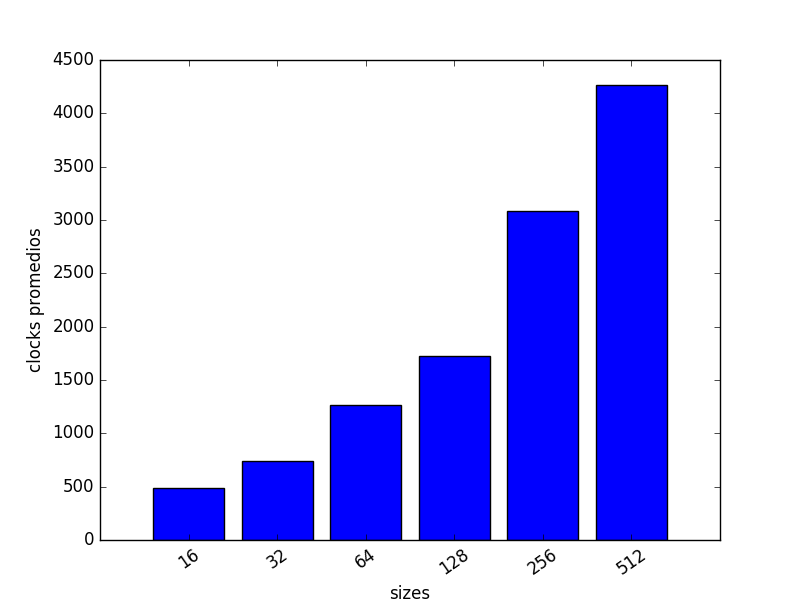
\includegraphics[width=.6\linewidth]{ClocksASMU.png}
    \caption{Código ASM con matriz U}
    \label{fig:ASMU}
\end{figure}

\pagebreak

\begin{figure}[h]
  \centering
    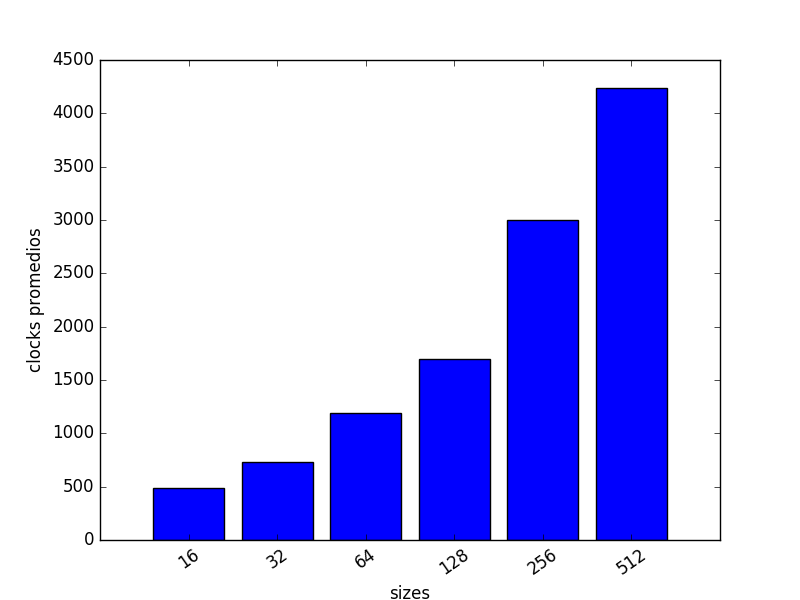
\includegraphics[width=.6\linewidth]{ClocksASMV.png}
    \caption{Código ASM con matriz V}
    \label{fig:ASMV}
  \centering
    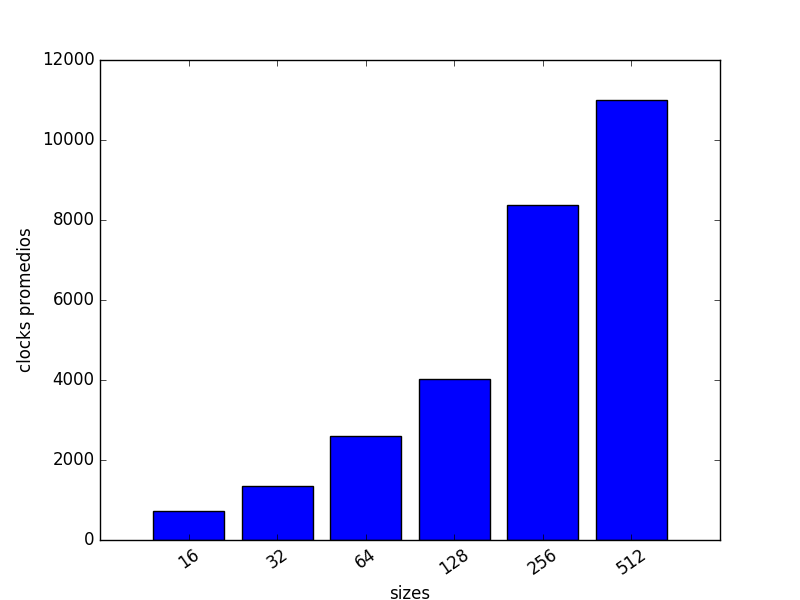
\includegraphics[width=.6\linewidth]{ClocksCU.png}
    \caption{Código C con matriz U}
    \label{fig:CU}
\end{figure}

\begin{figure}[h]
  \centering
    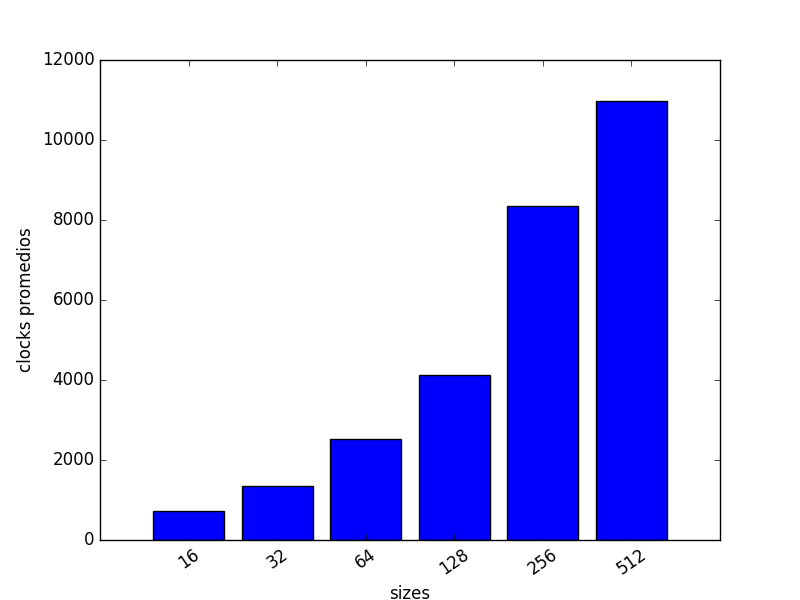
\includegraphics[width=.6\linewidth]{ClocksCV.png}
    \caption{Código C con matriz V}
    \label{fig:CV}
\end{figure}

\pagebreak

\subsection{solver\_project}

En $solver_project$ se realizaron 1000 ejecuciones de nuestro c\'odigo en ASM y nuestro c\'odigo en C, con las correspondientes optimizaciones O0, O2, O3. Las ejecuciones se realizaron para distintos tamaños de matrices.
Los tamaños que utilizamos fueron de 128x128, 256x256 y 512x512.
En cada ejecuci\'on, tomamos los tiempos de corrida del algoritmo, para poder utilizarlos para realiar gr\'aficos, para poder ver de manera mas clara cual es el rendimiento de nuestro c\'odigo en ASM comparado con el c\'odigo en C.
Las mediciones realizadas las almacenamos en un archivo csv, el cual utilizamos para realizar los gr\'aficos mencionados anteriormente.
Los gr\'aficos los realizamos utilizando codigo Python, con las bibliotecas Numpy y Matplotlib.
En los gr\'aficos, expuestos a continuaci\'on, podemos observar que nuestra hip\'otesis se cumple.
Es clara la superioridad de performance del codigo ASM con operaciones SIMD, a comparaci\'on de C.
Y lo que podemos ver es que por mas que utilicemos las distintas optimizaciones para compilar el c\'odigo C, igualmente el codigo ASM sigue siendo mas performante.

\begin{figure}[h]
  \centering
    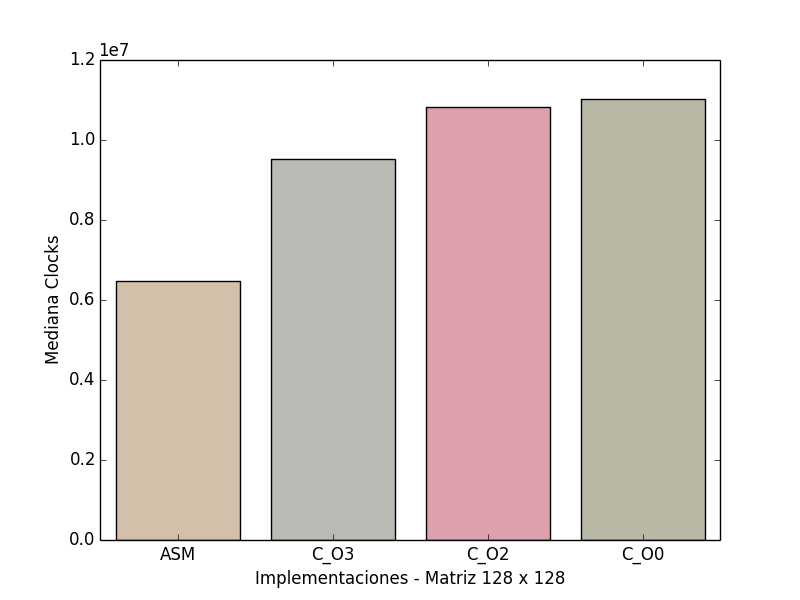
\includegraphics[width=.6\linewidth]{128x128.png}
    \caption{Tiempos para Matriz 128x128}
    \label{fig:M128}
\end{figure}

\pagebreak

\begin{figure}[h]
  \centering
    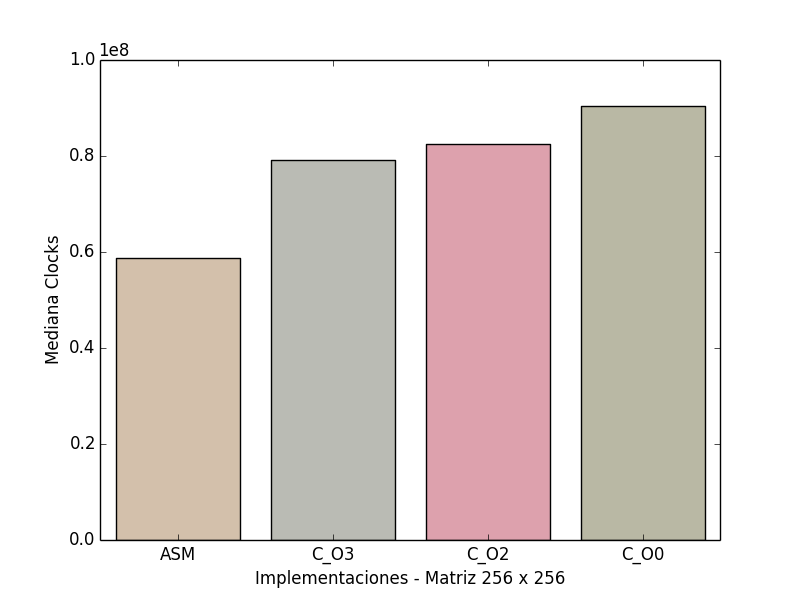
\includegraphics[width=.6\linewidth]{256x256.png}
    \caption{Tiempos para Matriz 256x256}
    \label{fig:M256}
\end{figure}

\begin{figure}[h]
  \centering
    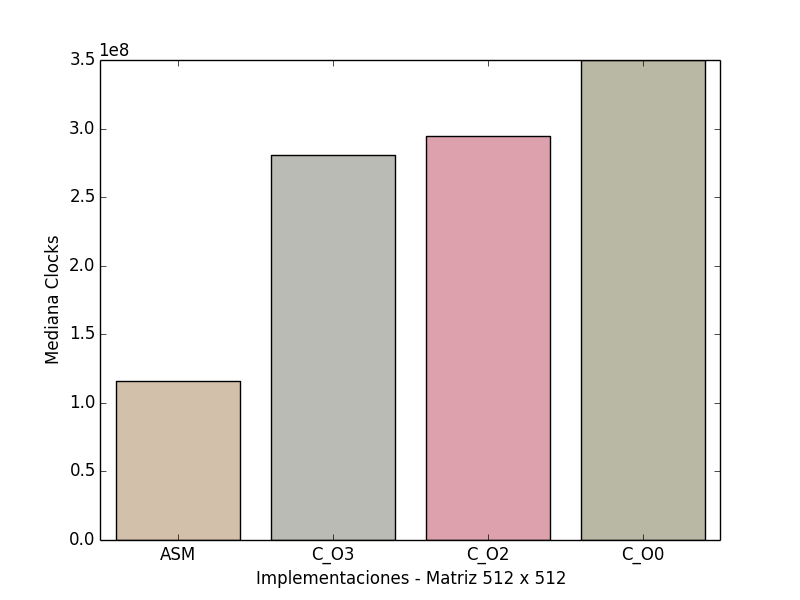
\includegraphics[width=.6\linewidth]{512x512.png}
    \caption{Tiempos para Matriz 512x512}
    \label{fig:M512}
\end{figure}

